\documentclass[12pt]{article}
\usepackage{hhline}
\usepackage{graphicx}
\graphicspath{{pictures/}}
\DeclareGraphicsExtensions{.png}
\usepackage{multirow}
\usepackage{amsmath}
\usepackage{mathtext}
\usepackage[T2A]{fontenc}
\usepackage[utf8]{inputenc}
\usepackage{pscyr} 
\usepackage[ left=2cm,right=2cm, top=1.5cm,bottom=1cm,bindingoffset=0cm]{geometry}

\begin{document}
\pagestyle{empty}
\begin{center}
\large{\textbf{Университет ИТМО}}
\end{center}
\rule{500pt}{1pt}
\par\bigskip\par\bigskip\par\bigskip\par\bigskip\par\bigskip\par\bigskip\par\bigskip\par\bigskip
\begin{center}
\Large
\textbf{Отчёт по лабораторной работе №4}

\textbf{\textit{«Изучение свойств идеального газа на примере воздуха»}}


\end{center}
\par\bigskip\par\bigskip\par\bigskip\par\bigskip\par\bigskip\par\bigskip\par\bigskip\par\bigskip\par\bigskip\par\bigskip\par\bigskip\par\bigskip\par\bigskip\par\bigskip      
\begin{flushright}
\large
Выполнил: Федюкович С. А.
\par\bigskip
Факультет: МТУ “Академия ЛИМТУ”
\par\bigskip
Группа: S3100                       
\par\bigskip\par\bigskip\par\bigskip

\rule{150pt}{0.5pt}
\par\bigskip\par\bigskip\par\bigskip\par\bigskip                                                            
 Проверил: Пшеничников В. Е. 
\par\bigskip \par\bigskip

\rule{150pt}{0.5pt}
\end{flushright}
\par\bigskip\par\bigskip\par\bigskip\par\bigskip\par\bigskip\par\bigskip\par\bigskip\par\bigskip\par\bigskip\par\bigskip     
\begin{center}
\large
Санкт-Петербург
\par\bigskip
2018
\end{center}
\newpage

\section*{Цель работы}
\begin{enumerate}
\item Экспериментальная проверка уравнения состояния идеального газа.
\item Определение температуры абсолютного нуля по шкале Цельсия.
\end{enumerate}
\section*{Теоретические основы лабораторной работы}

В том случае, когда состояние  газа далеко от области фазовых превращений, его с достаточной  степенью точности можно считать идеальным. В качестве идеального газа в работе используется  обычный атмосферный воздух.

Для произвольной массы m идеального газа справедливо следующее уравнение состояния;
\begin{equation}
pV = \frac{m}{\mu}RT,
\end{equation}	 	
где $p$ --- давление, $V$ --- объем, $\mu$ --- молярная масса, $T$ --- абсолютная температура газа, $R$ --- универсальная  газовая  постоянная.
Это  уравнение  называется уравнением Менделеева-Клапейрона. 

Нулю абсолютной температуры по шкале Цельсия соответствует значение $273,15 ^{\circ}C$. Градусы шкалы абсолютной температуры (шкалы Кельвина) и шкалы Цельсия выбраны одинаковыми. Поэтому значение абсолютной температуры связано со значением температуры по шкале Цельсия формулой:
\begin{equation}
T(K) = t(^{\circ} C) - t_{o}=t(^{\circ}C)+273,15 ^{\circ}C.
\end{equation}

\begin{center}
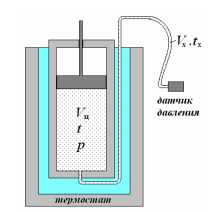
\includegraphics{1}
\end{center}
Пусть исследуемый газ находится в цилиндре с контролируемым рабочим объемом $V_{ц}$, масса газа в цилиндре $m_{ц}$. Температура $t$ цилиндра с газом поддерживается постоянной.

Датчик давления, работающий при комнатной температуре, вынесен за пределеы рабочего объёма и соединён с последним трубкой. Объём газа $V_{x}$ в этой трубке мал по сравнению с рабочим объёмом $V_{ц}$. В соединительной трубке также находится газ массой $m_{x}$ при некоторой неизвестной средней температуре $t_{x}$,  лежащей в интервале от комнатной температуры до температуры $t$ рабочего объёма.

В работе измеряется зависимость давления p газа от велечины рабочего объёма $V_{ц}$ при разных значениях температуры $t$ (от $20^{\circ} C$ до  $60^{\circ} C$). Выведем соотношение, связывающее рабочий объём и давление газа при постоянной температуре. Общее количество вещества в рабочем объёме и соединительной трубке в течение всей работы остаётся постоянным.
\begin{equation}
v = (m_{ц}+m_{x})/\mu
\end{equation}			

Выражая массы газа $m_{ц}$ и $m_{x}$ из уравнения состояния $(1)$, абсолютную температуру из соотношения $(2)$, и подставляя найденные выражения в формулу $(3)$, получим:
\begin{equation}
v = \frac{pV_{ц}}{R(t-t_{o})} +\frac{pV_{x}}{R(t_{x}-t_{o})} 
\end{equation}			
Из этого уравнения найдем искомое соотношение:
\begin{equation}
V_{ц} = \frac{vR(t-t_{o})}{p}-\frac{V_{x}(t-t_{o})}{(t_{x}-t_{o})} 
\end{equation}

Из-за перераспределения газа между объёмами $V_{ц}$ и   в процессе измерения температура   может изменяться. Однако, при относительно малой величине   изменением второго слагаемого в формуле $(5)$ можно пренебречь. Поэтому при неизменной температуре $t$ зависимость рабочего объёма $V_{ц}$ от обратного давления $1/p$ является линейной. 
\begin{equation}
K = vR(t-t_{o}),
\end{equation}

Угловой коэффициент этой зависимости в свою очередь, линейно меняется с температурой и обращается в нуль при абсолютном нуле температур. Таким образом, изучение зависимости $К(t)$ позволяет найти значение $t_{o}$.

Рассмотрим другой, более точный, способ определения величины $t_{o}$. Если для разных температур измерение давления проводить при одних и тех же значениях объёма, то полученные данные легко преобразуются в зависимость давления от температуры при разных значения рабочего объёма газа. Теоретический вид этой зависимости получается из уравнения $(5)$:
\begin{equation}
p=\frac{vR(t-t_{o})}{V_{ц}(1+x(t))}\approx \frac{vR(t-t_{o})}{V_{ц}}(1+x(t)),
\end{equation}
где $x(t)=\frac{V_{x} (t-t_{o})}{V_{ц} (t_{x}-t_{o} ) }$. Справедливость приближенного равенства в формуле (7) обусловлена тем, что значения функции $x(t)$  малы, и для малых x можно воспользоваться формулой приближенных вычислений:
\begin{equation}
(1+x)^{\alpha} \approx 1 + \alpha x.
\end{equation}
В данном случае $\alpha = -1$.

\begin{center}
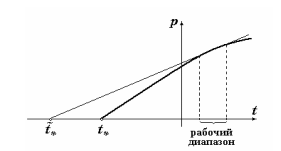
\includegraphics{2}
\end{center}
При неизменном рабочем объёме $V_{ц}$ график зависимости давления от температуры в соответствии с формулой $(7)$ должен быть почти линейным. Причем давление должно обращаться в нуль как раз при $t = t_{o}$ . Из-за малости функции $x(t)$ отклонение от линейности невилико, и при измерении в ограниченном диапазоне температур практичечки незаметно. Но, если искать значение  $t_{o}$  с помощью линейной аппроксимации экспериментальной зависимости $p(t)$, экстраполируя аппроксимирующую прямую до пересечения с осью $t$, то найденное приближенное значение   окажется систематически смещённым влево относительно истинного значения   . Причина этого в следующем. Величина $x(t)$ в первом приближении линейно растущая функция температуры, с учетом этого график функции $p(t)$ из уравнения $(7)$ оказывается параболой выпуклой вверх. Аппроксимирующая прямая, параметры которой найдены по точнкам в рабочем диапазоне температур, идет практически по касательной к этому графику, «промахиваясь» мимо истинного значения  , как изображено на рис. 1. Однако, можно показать, что разность  при малом отношении $V_{x}/V_{ц}$  должна убывать обратно пропорционально объёму $V_{ц}$. Поэтому, правильное значение температуры абсолютного нуля может быть найдено как предел:
\begin{equation}
t_{o} = \lim_{1/V_{ц}\to 0}\widetilde{t}_{o}
\end{equation}
линейным продолжением графика зависимости  $\widetilde{t}_{o}$ от $1/V_{ц}$ к значению $1/V_{ц} =0$.
\section*{Экспериментальные данные}
Приборные погрешности $\Delta V = 1$ мл, $\Delta p = 0,1$ кПа.

Атмосферное давление $p_{0}$ , определённое с помощью лабораторного барометра равно 756.8 мм ртутного столба.
\begin{table}[h!]
\begin{center}
Таблица 1.1. Зависимость давления от объёма при температуре  $t_{3}=20^{\circ} C$

\begin{tabular}{|c|c|c|c|c|c|}
\hline
№ &	$V_{ц}$, мл	&$\Delta p_{1}$ , кПа	&$\Delta p_{2}$, кПа	&$P$, кПа&	$1/p$, кПа \\
\hline
1&		50&		32,3	&	32,3&		132,8&		0,008\\
\hline
2&	        60&		12,8&		15,2&		114,5	&	0,009\\
\hline
3&		70&		-1,8&		0&		99,6	&	0,010\\
\hline
4&		80&		-12,1&		-11,9	&	88,5	&	0,011\\
\hline
5&		90&		-21,2&		-21,3&		79,2&		0,013\\
\hline
6&		100&		-28,8&		-28,8	&	71,7	&	0,014\\
\hline
7&		110&		-35,2&		-35,3	&	62,2	&	0,015\\
\hline
8	&	120	&	-40,6	&	-36,8&		59,9&		0,017\\
\hline
\end{tabular}
\end{center}
\end{table} 
\begin{table}[h!]
\begin{center}
Таблица 1.2. Зависимость давления от объёма при температуре $t_{3}=30^{\circ} C$
\begin{tabular}{|c|c|c|c|c|c|}
\hline
№ &	$V_{ц}$, мл	&$\Delta p_{1}$ , кПа	&$\Delta p_{2}$, кПа	&$P$, кПа&	$1/p$, кПа \\
\hline
1&		50&		53,4&		53,4&		153,9	&	0,0065\\
\hline
2	&	60	&	29,5&		29&		129,7&		0,0077\\
\hline
3&		70	&	13,7&		9,7	&	112,2&		0,0089\\
\hline
4&		80	&	-0,9&		-3,5&		98,3&		0,0102\\
\hline
5	&	90	&	-11,7&		-13,7&		87,8&		0,0114\\
\hline
6&		100&		-22,4&		-22,5&		78,0&		0,0128\\
\hline
7	&	110&		-30,8&		-30,8	&	69,7&		0,0143\\
\hline
8&		120&		-36,8	&	-36,8	&	63,7	&	0,0157\\
\hline
\end{tabular}
\end{center}
\end{table} 
\newpage
\begin{table}[h!]
\begin{center}
Таблица 1.3. Зависимость давления от объёма при температуре  $t_{3}=40^{\circ} C$

\begin{tabular}{|c|c|c|c|c|c|}
\hline
№ &	$V_{ц}$, мл	&$\Delta p_{1}$ , кПа	&$\Delta p_{2}$, кПа	&$P$, кПа&	$1/p$, кПа \\
\hline
1&		50&		50,2&		51,7&		151,4&		0,0066\\
\hline
2&		60&		28&		27,6&		128,3&		0,0078\\
\hline
3&		70&		3,7	&	5,1&		104,9	&	0,0095\\
\hline
4&		80&		-7,8&		-6,1&		93,5&		0,0107\\
\hline
5&		90&		-16,3	&	-16,5	&	84,1&		0,0119\\
\hline
6&		100&		-24,4&		-24,5&	76,0&		0,0132\\
\hline
7&		110&		-31,1&		-31,1	&	69,4	&	0,0144\\
\hline
8&		120&		-36,7	&	-36,7	&	63,8	&	0,0157\\
\hline
\end{tabular}
\end{center}
\end{table} 
\section*{Обработка результатов измерений}
\begin{enumerate}
\item	Переведем показания лабораторного барометра из миллиметров ртутного столба в паскали:
\begin{equation}
p_{0}(Па)= p_{0}(мм.рт.ст) 10^{-3} \frac{м}{мм} \rho g = 100495 (Па) = 100,495(кПа).
\end{equation}
Здесь $\rho = 13,55 \cdot 10^3  кг/м^3$ --- плотность ртути, $g = 9,819 м/c^2$ --- ускорение свободного падения на широте Санкт-Петербурга.

\itemДля каждой из 1.1 — 1.3  вычислим давление газа $p$ по формуле 
 \begin{equation}
p=p_{0} + \frac{\Delta p_{1} + \Delta p_{2}}{2} ,
\end{equation}
обратное давление 1/p и заполним пятую и шестую колонки таблиц.

\item По данным таблиц 1.1 — 1.3 для температур  построим на одной координатной сетке графики зависимости рабочего объёма $V_{цот}$ обратного давления $1/p$ . 
\newpage
Рис. 2. Графики зависимости рабочего объёма $V_{ц}$ от обратного давления $1/p$. 
Из рис. 2 видно, что зависимость $V_{ц}$ от $1/p$ во всех пяти случаях является прямолинейной. Кроме того, наблюдается рост углового коэффициента $K$ c ростом $t$.
\itemПеренесём значения рабочих температур   во второй столбец таблицы 2.1. Для каждого из графиков $V_{ц}$ от $1/p$ рассчитаем угловой коэффициент $K$, следующим образом:   
Пусть $X_{1},X_{2}$...$X_{n}$  --- абсциссы, $Y_{1},Y_{2}$...$Y_{n}$ --- ординаты графика некоторой
экспериментально измеренной зависимости $Y(X)$ . Если предполагается, что
эта зависимость линейна, т.е. $Y(X) = AX + C$, то наиболее вероятные
значения углового коэффициента $A$ и свободного слагаемого $C$ можно найти
из требования минимальности суммы квадратов отклонений ординат
экспериментальных точек от искомой прямой:
\begin{equation}
\sum_{i=1}^N( Y_{i} - (AX_{i} + C))^2 = min.
\end{equation}
Исходя из условия (15) можно получить следующие выражения
\begin{equation}
A = \frac{1}{D}\sum_{i=1}^N( X_{i} - \overline{X}) Y_{i}, C = \overline{Y} - A\overline{X},
\end{equation}
где 
\begin{equation}
\overline{X}=\frac{\sum_{i=1}^N X_{i}}{N},\overline{Y}=\frac{\sum_{i=1}^N Y_{i}}{N},D=\sum_{i=1}^N (X_{i} - \overline{X})^2.
\end{equation}
Погрешности коэффициента и слагаемого вычисляются по формулам:
\begin{equation}
\Delta A = \sqrt{E/D}, \Delta C = \sqrt{(\frac{1}{N} + \frac{\overline{X^2}}{D})E},
\end{equation}
где  
\begin{equation}
E=\frac{1}{N-2}\sum_{i=1}^N (Y_{i} - AX_{i} -C)^2.
\end{equation}
Значения $К$ занесём в таблицу 2.1:
\begin{table}[h!]
\begin{center}
\begin{tabular}{|c|c|c|}
\hline
№&	$t,^{\circ}C$&	$K$, Дж\\
\hline
1&	20&	7622\\
\hline
2&	30	&7585\\
\hline
3&	40&	7718\\
\hline
4&	50&	8084\\
\hline
5&  60	&       8513\\
\hline
\end{tabular}
\end{center}
\end{table} 	
\newpage
\itemПо таблице 2.1. построим график зависимости $K(t)$: 

\par\bigskip\par\bigskip\par\bigskip\par\bigskip\par\bigskip\par\bigskip\par\bigskip\par\bigskip\par\bigskip\par\bigskip\par\bigskip\par\bigskip\par\bigskip\par\bigskip\par\bigskip\par\bigskip\par\bigskip\par\bigskip\par\bigskip\par\bigskip\par\bigskip\par\bigskip\par\bigskip\par\bigskip\par\bigskip\par\bigskip\par\bigskip\par\bigskip            
Рис. 3. График зависимости углового коэффициента $К$  графика $V_{ц}(1/p)$ от температуры газа.
Как видим, в соответствии с формулой $(6)$ график «идёт» прямолинейно.
В теории график должен пересекать ось $t$ при температуре абсолютного нуля. По найденным экспериментальным точкам найдём угловой коэффициент $A$ и свободное слагаемое $C$ для зависимости $K(t)$ по формулам $(13), (14)$.

	$A = 23 $(Дж/$^{\circ}C$);
	$C = 6992,15 $(Дж);

Рассчитаем температуру абсолютного нуля:
 $t_{o} = \frac{-C}{A}=-306,5(^{\circ}C)$;
 
Вычислим погрешность температуры абсолютного нуля: 
$\Delta t_{o} = t_{o} \sqrt{\frac{\Delta A}{A}^2+\frac{\Delta C}{C}^2}  = -77,9^{\circ}C;$
		  
Таким образом, доверительный интервал найденного значения температуры абсолютного нуля: 
 $t_{o}= 306,5.5 \pm 77,9(^{\circ}C).$

\itemПо данным таблиц 1.1 – 1.5 заполним таблицу 2.2:

\begin{table}[h!]
\begin{center}
\begin{tabular}{|c|c|c|c|c|c|c|c|c|}
\hline
$V_{ц}$, мл	&50&	60	&70&	80&	90	&100&	110&	120\\
\hline
$T, ^{\circ}C	$&\multicolumn{8}{|c|}{$P$, кПа}\\
\hline
20&	132,8&	114,5&	99,6&	88,5	&       79,25	&71,7	&65,25&	59,9\\
\hline
30	&153,9&	129,75&	112,2&	98,3&	87,8&	78,05&	69,7&	63,7\\
\hline
40	&151,45	&128,3&	104,9&	93,55&	84,1	&       76,05&	69,4&	63,8\\
\hline
$1/V_{ц}, мл^{-1}$ &0,02	&0,017&	0,014&	0,013&	0,011	&0,01&	0,009&	0,0083\\
\hline
$\widetilde{t_{o}}$ , C&	-205,22&	-192,91&	-219,75	&-235,1&	-232,092&	-246,442	&-225,788	&-251,691\\
\hline
\end{tabular}
\end{center}
\end{table} 
\newpage
Пользуясь таблицей 2.2 для значений объема цилиндра 50, 90, 120 мл на одной координатной сетке построим графики $p(t)$:
\par\bigskip\par\bigskip\par\bigskip\par\bigskip\par\bigskip\par\bigskip\par\bigskip\par\bigskip\par\bigskip\par\bigskip\par\bigskip\par\bigskip\par\bigskip\par\bigskip\par\bigskip\par\bigskip\par\bigskip\par\bigskip\par\bigskip\par\bigskip\par\bigskip\par\bigskip\par\bigskip\par\bigskip\par\bigskip\par\bigskip\par\bigskip\par\bigskip 
Рис. 4. Графики зависимости давленияи от температуры. Как видим, графики «идут» прямолинейно.


\item Для каждого из объемов (покажем рассчеты только для $V_{1}  = 50 $мл) в таблице 2.2 найдём значение обратного объема $1/V_{ц}$ и рассчитаем величину $\widetilde{t_{o}}$  по формуле: \\
$\widetilde{t_{o}} = - \frac{c}{a} = -205,219^{\circ}C$,

где $a$ и $c$ , соответственно, угловой коэффициент и свободное слагаемое для зависимости $p(t)$, вычисляемые по формулам $(13), (14)$.
Занесём значения в таблицу 2.2.
\newpage
\itemПользуясь таблицей 2.2, по формулам $(13), (14)$ найдём угловой коэффициент $A\rq{}$   и свободное слагаемое $C\rq{}$ для зависимости  $\widetilde{t_{o}}(1/V_{ц})$. Величина $C\rq{}$ фактически есть предел $(9)$, т.е. совпадает со значением $t_{o}$. На координатной сетке  $\widetilde{t_{o}}$ от $1/V_{ц} $ отметим экспериментальные
точки и проведём прямую, соответствующую найденным параметрам $A\rq{}$   и $C\rq{}$ . Продолжим прямую до пересечения с осью ординат.
\par\bigskip\par\bigskip\par\bigskip\par\bigskip\par\bigskip\par\bigskip\par\bigskip\par\bigskip\par\bigskip\par\bigskip\par\bigskip\par\bigskip\par\bigskip\par\bigskip\par\bigskip\par\bigskip\par\bigskip\par\bigskip\par\bigskip\par\bigskip\par\bigskip\par\bigskip\par\bigskip\par\bigskip\par\bigskip\par\bigskip\par\bigskip\par\bigskip 
Рис. 5. Зависимость  $\widetilde{t_{o}}(1/V_{ц})$. Точка пересечения с осью ординат есть температура абсолютного нуля  $t_{o}$.

\itemРассчитаем погрешность  $\Delta t_{o}$  как  $\Delta C\rq{}$  по формулам $(15)–(16)$.\\
$A\rq{} = 4151 (^{\circ}C/мл^{-1} )$\\
$C\rq{} = -279 (^{\circ}C)$;\\
Вычислим погрешность температуры абсолютного нуля:\\
$\Delta C= \sqrt{(\frac{1}{N} + \frac{\overline{X^2}}{D})E}\approx 14,48^{\circ}C$.
\end{enumerate}
\section*{Вывод}
Мы убедились, что зависимость объёма от величины обратного давления является линейной, а значит объём обратно пропорционален давлению при неизменной температуре, что согласуется с уравнением состояния идеального газа:$pV = \frac{m}{\mu}RT$.

Помимо этого мы рассчитали температуру абсолютного нуля двумя способами. Первый способ, основан на том, что угловой коэффициента $K$ графика зависимости объёма от обратного давления обращается в нуль при температуре абсолютного нуля. Второй способ построен на анализе зависимости давления от температуры при постоянном объёме: при различных значениях объёма определяется $\widetilde{t_{o}}$ --- приближенное значение температуры абсолютного нуля. 
Затем это значение уточняется как предел   при $1/V_{ц} \to 0$. Как и ожидалось, этот способ дал более точный результат $ t_{o}=-279\pm14,5(^{\circ}C)$.

Тот факт, что полученные значения достаточно близки, подтверждает правильность расчетов и рассуждений, на основе которых были произведены расчеты. 


\end{document}